% Create a cropped pdf and convert it to svg
% The program pdf2svg must be installed
% Run pdflatex -shell-escape
% Convert resulting svg to png with
% inkscape -z -d=250 -e model.png model.svg
% Where 250 is the pixel density 
\documentclass[crop,tikz,convert={outext=.svg,
			   command=\unexpanded{pdf2svg 
			  \infile\space\outfile}},multi=false]{standalone}

\usepackage{siunitx}

\usetikzlibrary{positioning, arrows} 
\usetikzlibrary{shapes.geometric, shapes.multipart}

\begin{document}

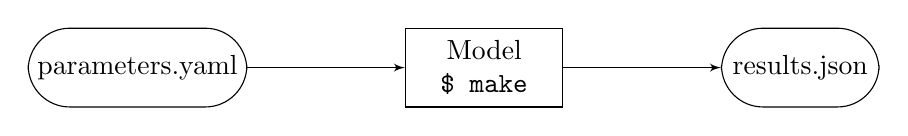
\begin{tikzpicture}[>=latex']
    \tikzset{block/.style = {draw, rectangle, align=center, minimum width = 2cm, minimum height = 1cm},
             io/.style = {draw, shape=rectangle, rounded corners=1.5em, align=center,
                                minimum width = 2cm, minimum height = 1cm}
            }
    \node (params) [io] {parameters.yaml};
    \node (model) [block, right =2cm of params] {Model \\ \texttt{\$ make}};
    \node (results) [io, right =2cm of model] {results.json};
    \path[draw, ->] (params) edge (model);
    \path[draw, ->] (model) edge (results);
\end{tikzpicture}

\end{document}
